\documentclass[a4paper,11pt,dvipdfmx]{ujarticle}
% パッケージ
\usepackage{graphicx}
\usepackage{url}
\usepackage{float}
% レイアウト指定を記述したファイルの読み込み
\input{layout}
 
% タイトルと氏名を変更せよ．
\title{インターネットの利用状況}
\author{G684122026 チャンミャエキン}
 
\begin{document}
 
\maketitle
 
\section{デジタル競争力ランキング}%ここにタイトルが入る
 
国際経営開発研究所（IMD）の調査\cite{imd}によると，
図\ref{fig:ranking}に示すように，
日本のデジタル競争力は調査対象の64カ国中，総合で28位となっている．
また，知識分野では25位であり，
上位国と比較すると差が大きいことがわかる．
 
\begin{figure}[htbp]
    \centering
    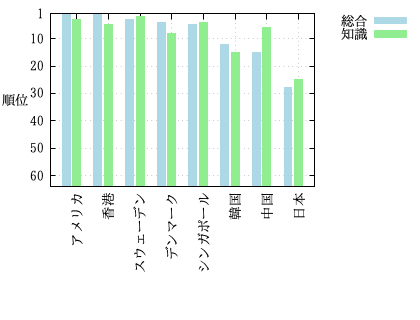
\includegraphics[width=0.7\linewidth]{fig31.png}
    \caption{デジタル競争力ランキング (64カ国中)}\label{fig:ranking}
\end{figure}
 
\section{ブロードバンドの整備状況}
 
OECDによるブロードバンド回線の普及に関する調査\cite{oecd}によると，
表\ref{tbl:broadband}に示すように，
日本における100人あたりのモバイルブロードバンドの加入者数は190.5で，
第1位になっている．
2位はエストニア(179.9)，3位は米国(169.0)と続いており，
日本の通信インフラの整備状況は世界的にも高い水準にあるといえる．
 
\begin{table}[htbp]
    \centering
    \caption{モバイルブロードバンドの加入者数 (100人あたり)}
    \label{tbl:broadband}
 
    \begin{tabular}{|c|l|r|}\hline
        順位 & 国名 & 加入者数 \\
        \hline
        1位 & 日本 & 190.5 \\
        \hline
        2位 & エストニア & 179.9 \\
        \hline
        3位 & 米国 & 169.0 \\
        \hline
        4位 & フィンランド & 157.0 \\
        \hline
        5位 & デンマーク & 141.7 \\
        \hline
        6位 & ラトビア & 141.6 \\
        \hline
        7位 & イスラエル & 139.9 \\
        \hline
        8位 & オランダ & 133.7 \\
        \hline
        9位 & ポーランド & 131.3 \\
        \hline
        10位 & スウェーデン & 127.2 \\
        \hline
    \end{tabular}
\end{table}
\section{考察}
 
以上の調査結果から，日本のデジタル化の状況について
次のようなことが考えられる．
\begin{itemize}
    \item モバイルブロードバンドの加入者数は世界第1位であり，
          通信インフラは非常に充実している．
    \item 一方で，IMDのデジタル競争力ランキングでは
          64カ国中28位にとどまっており，インフラの水準に対して
          活用の面で課題がある．
    \item この差は，デジタル技術を活用できる人材の不足や，
          企業・行政におけるデジタル化の遅れが
          原因の一つであると考えられる．
    \item 今後は，整備されたインフラを十分に活かすために，
          教育やビジネスの現場におけるデジタル人材の育成が
          重要な課題となる．
\end{itemize}
% ここから本文
% 節見出し: \section{}
% を使う
 
% 本文(1)
%  参考文献の参照: \cite{}
%  図番号の参照： \ref{}
% を使う
% 文献データベースのキーワードは oecd と imd
% になっている．
 
% 図の挿入
% \includegraphics{}
% を
% \begin{figure}[htbp]
% \end{figure}
% で囲み
% \caption{}
% で図のタイトルを入れる．
% \label{}
% を使って図番号が参照できるようにする
% また，
% \centering
% で図が中央に来るようにする
 
% ーーー
% 節見出し(2)
 
% 本文(2)
 
% 表の挿入
% \begin{tabular}
% \end{tabular}    
% による表の記述を
% \begin{table}[htbp]
% \end{table}
% で囲み
% \caption{}
% で表のタイトルを入れる．
% \label{}
% を使って表番号が参照できるようにする
% また，
% \centering
% で表が中央に来るようにする
 
% ーーー
% 見出し(3)
% 考察
%
% \begin{itemize}
% \end{itemize}
% を使って箇条書きで記述する
 
% ここに参考文献が入る
%
\bibliographystyle{junsrt}
\bibliography{exercise.bib}
 
\end{document}
has context menu


has context menu